\documentclass{beamer}
\mode<presentation>
%\mode<handout>

\beamertemplatenavigationsymbolsempty %remove navigation symbols

\usepackage[utf8]{inputenc}
\usepackage[ngerman]{babel}

\usepackage{tikz}
\usepackage{amsmath}
\usepackage{graphicx}

\title{OpenSCAD}
\author{Michael Stypa \\ mstypa@uni-osnabrueck.de}
\date{\today}

\begin{document}

\begin{frame}
  \titlepage
\end{frame}

\begin{frame}
  \frametitle{Boolesche Operatoren}
  \framesubtitle{in 2D}
  \begin{itemize}
    \item \begin{tikzpicture}[baseline=-1ex, fill=blue!50]
        % left hand
        \scope
        \clip (0,0) rectangle (0,0)
        (1,0) circle (1);
        \fill (0,0) circle (1);
        \endscope
        % right hand
        \scope
        \clip (0,0) rectangle (0,0)
        (0,0) circle (1);
        \fill (1,0) circle (1);
        \endscope
        % outline
        \draw (0,0) circle (1)
          (1,0) circle (1);
      \end{tikzpicture}
      Schnittmenge / intersection\quad
      $A \cap B$
    \item \begin{tikzpicture}[baseline=-1ex, fill=blue!50]
        % left hand
        \scope
        \clip (-1,-1) rectangle (2,1)
        (1,0) circle (1);
        \fill (0,0) circle (1);
        \endscope
        % right hand
        \scope
        \clip (0,-1) rectangle (2,1)
        (0,0) circle (1);
        \endscope
        % outline
        \draw (0,0) circle (1)
          (1,0) circle (1);
      \end{tikzpicture}
      Differenzmenge / difference\quad
      $A \setminus B$
    \item \begin{tikzpicture}[baseline=-1ex, fill=blue!50]
        \draw[fill] (0,0) circle (1)
          (1,0) circle (1);
      \end{tikzpicture}
      Vereinigungsmenge / union\quad
      $A \cup B$
  \end{itemize}
\end{frame}

\begin{frame}
  \frametitle{Constructive Solid Geometry (CSG)}
  \framesubtitle{oder Konstruktive Festkörpergeometrie}
    \begin{tikzpicture}[level 1/.style={sibling distance=6cm, level distance=1.5cm}, level 2/.style={sibling distance=3cm, level distance=3cm}]
    \node {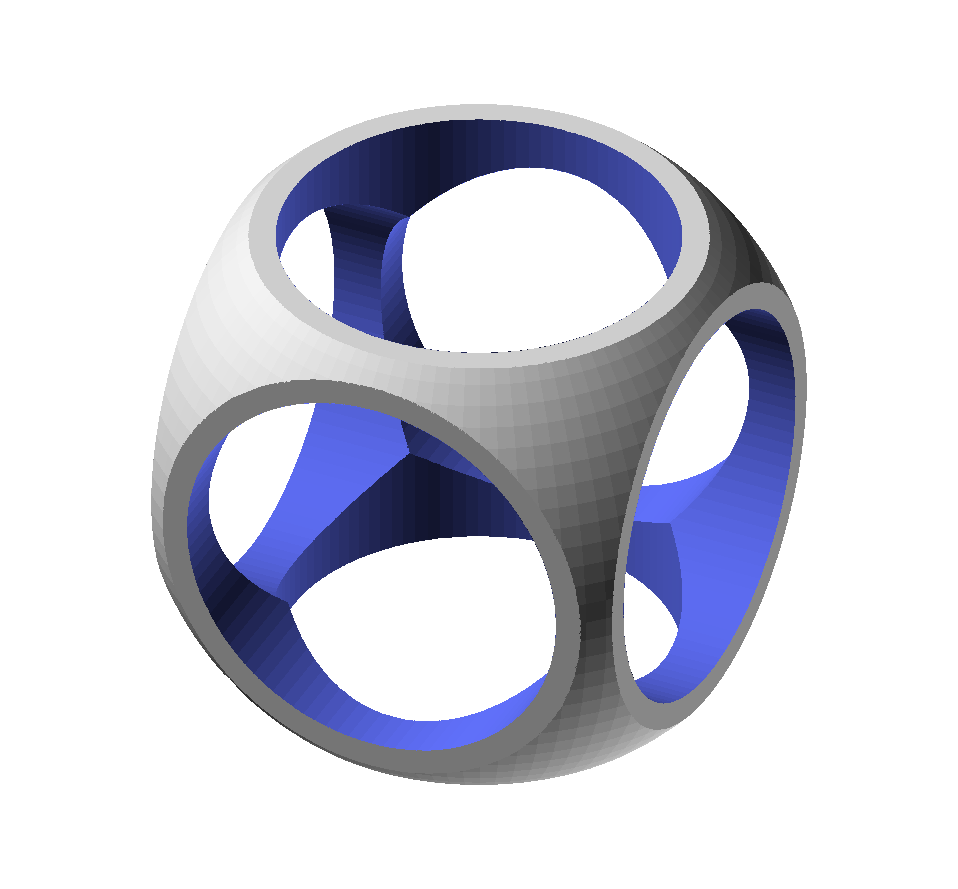
\includegraphics[scale=0.09]{models/full.png}}
      child{ node{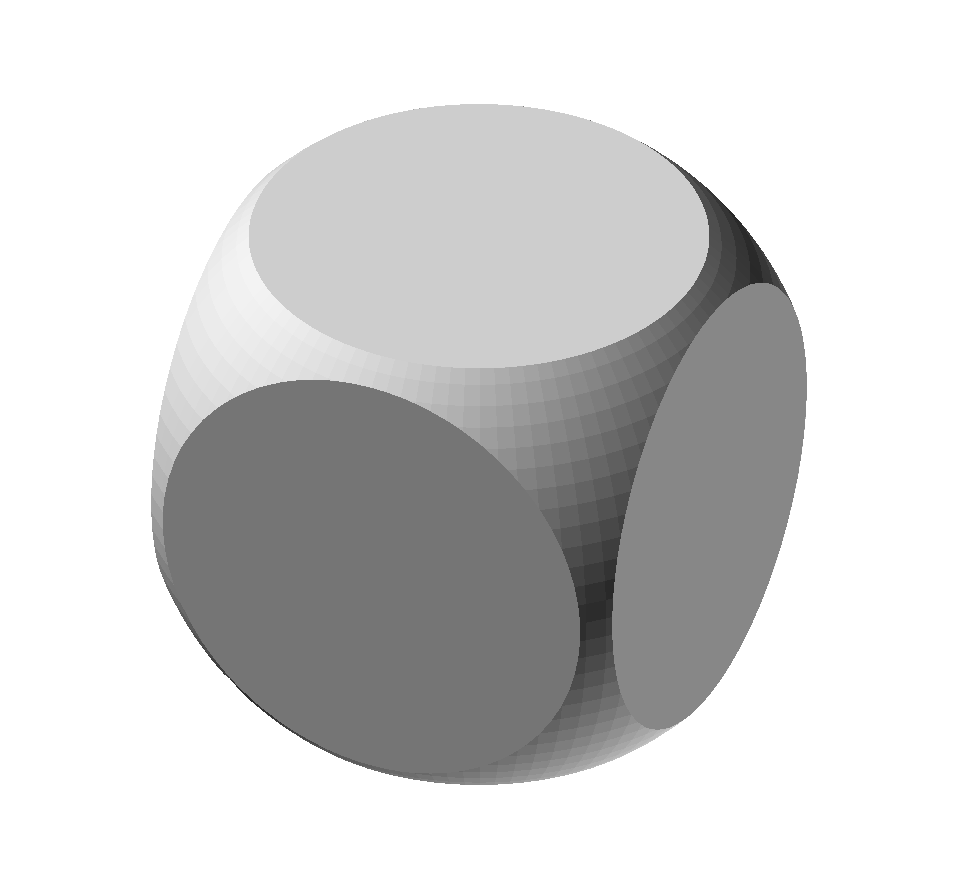
\includegraphics[scale=0.09]{models/cutsphere.png}}
        child {node{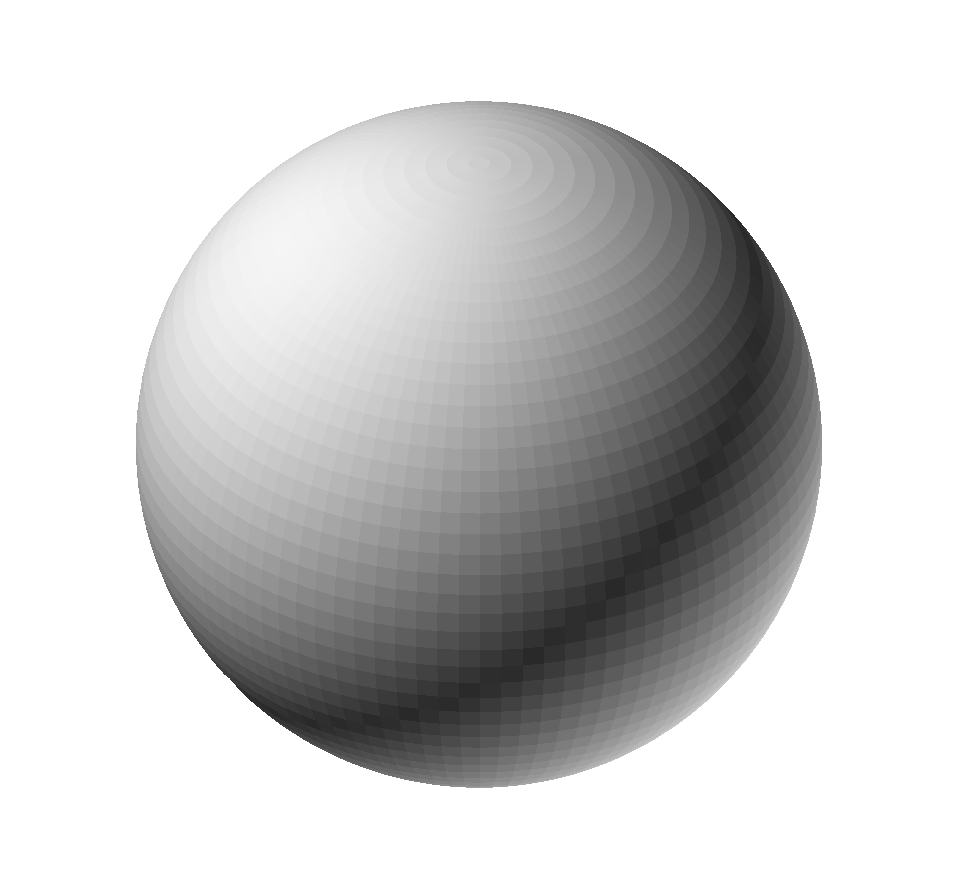
\includegraphics[scale=0.09]{models/sphere.png}}}
        child {node{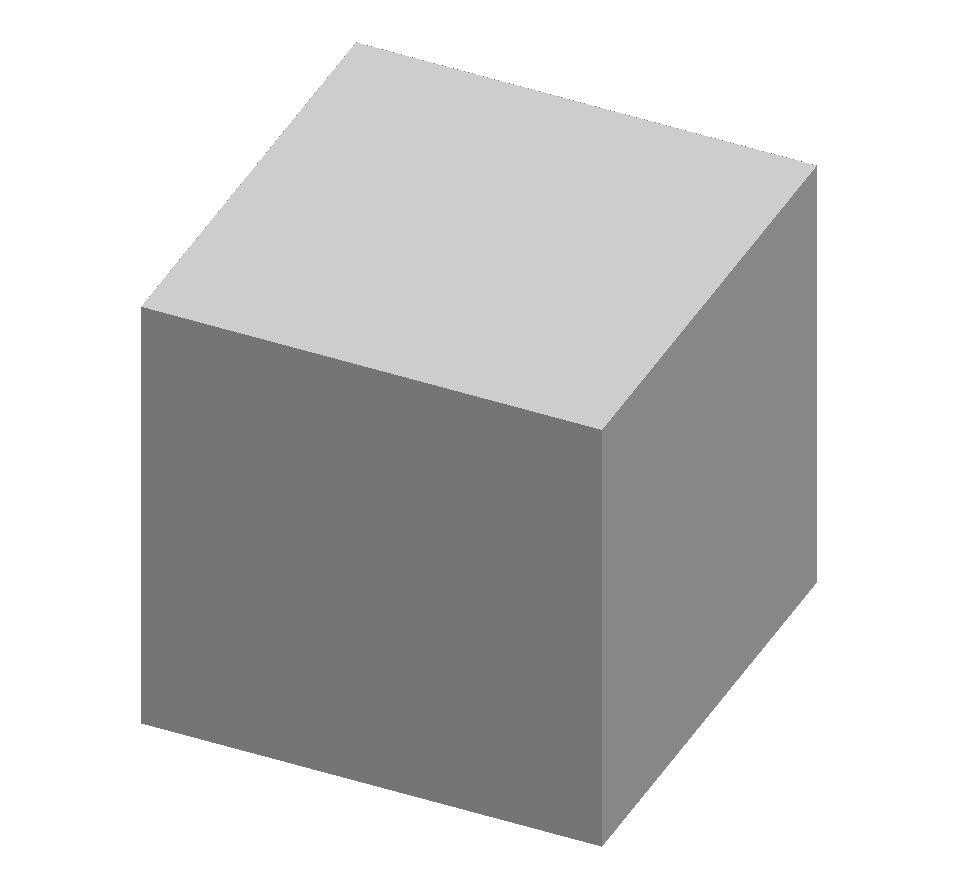
\includegraphics[scale=0.09]{models/box.png}}}
      }
      child{ node{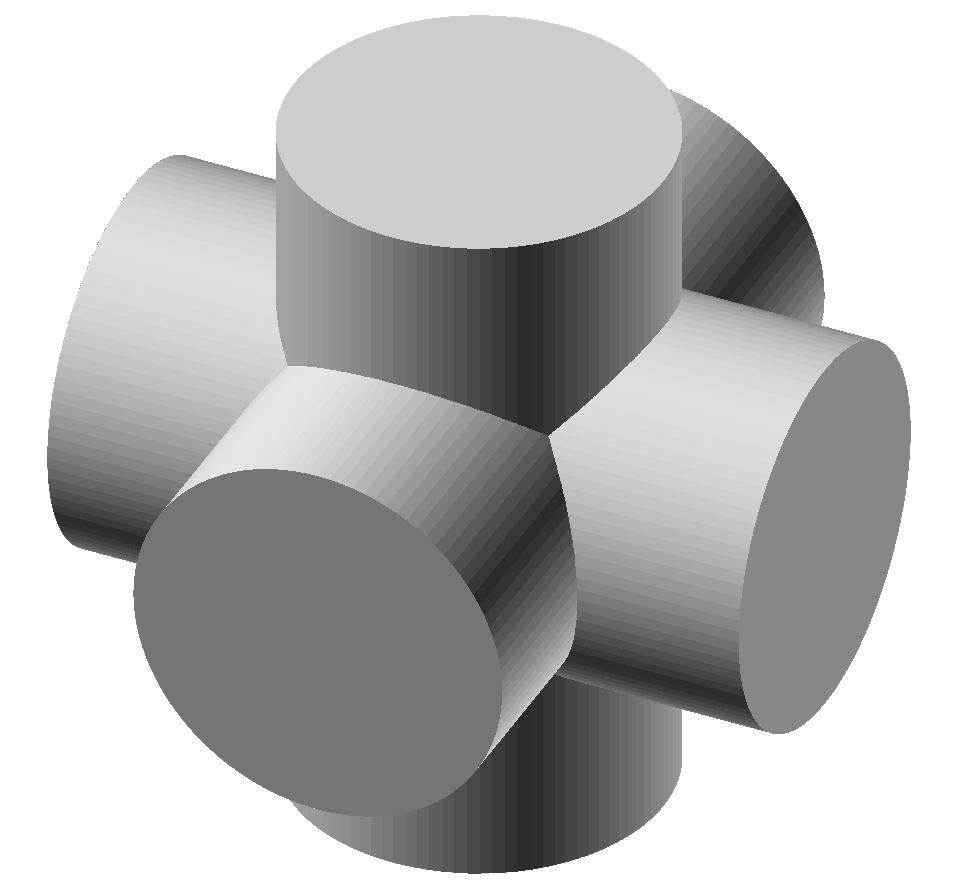
\includegraphics[scale=0.09]{models/cross.png}}
        child {node{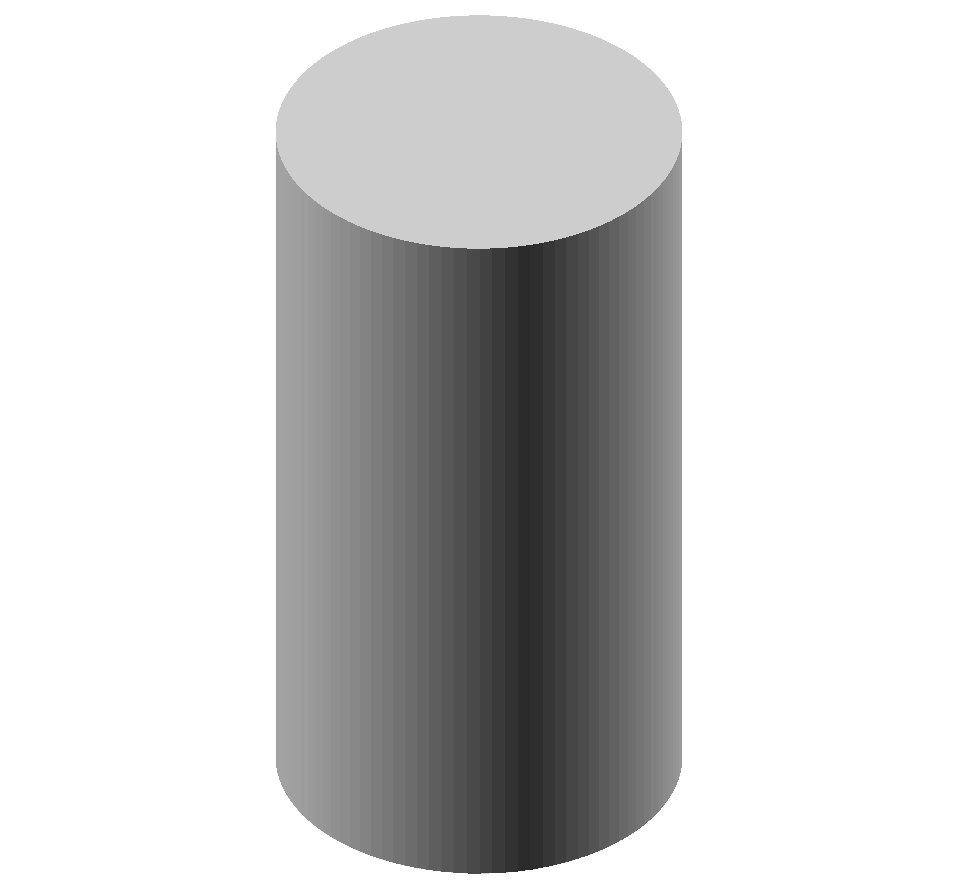
\includegraphics[scale=0.09]{models/cylinder.png}}}
        child {node{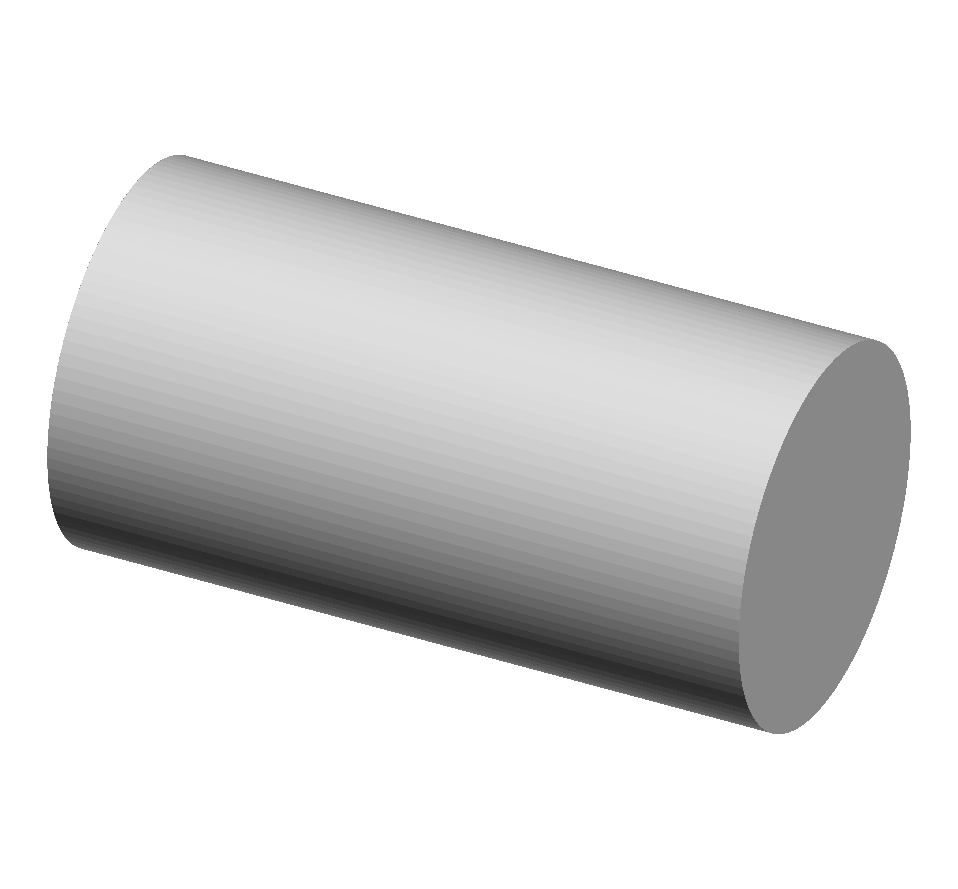
\includegraphics[scale=0.09]{models/rotcylinder.png}}}
      }
      ;
  \end{tikzpicture}
\end{frame}

\end{document}
